%Template elaborado por Alma Rocío Sagaceta Mejía

\documentclass[twoside]{article} %tipo de documento y a dos columnas

%Paquetería que se usan para la elaboración de la práctica
\usepackage{amssymb}
\usepackage[table,xcdraw]{xcolor}
\usepackage{amsmath}
\usepackage[spanish]{babel}
\usepackage[utf8x]{inputenc}
\usepackage[sc]{mathpazo} 
\linespread{1.05}
\usepackage{microtype}
\usepackage[hang, small,labelfont=bf,up,textfont=it,up]{caption}
\usepackage{lettrine}
\usepackage{graphicx}
\usepackage[hmarginratio=1:1,top=20mm,bottom=35mm,right=15mm,left=15mm,columnsep=20pt]{geometry}
\usepackage{multicol} 
\usepackage{booktabs}
\usepackage{float} 
\usepackage{subfigure}
\usepackage{paralist} 
\usepackage{hyperref} 
\usepackage{abstract}
\usepackage{titlesec}
\usepackage{fancyhdr} 

%Renombrar comandos
\renewcommand{\abstractnamefont}{\normalfont\bfseries}
\renewcommand{\abstracttextfont}{\normalfont\small\itshape}
\renewcommand\thesection{\Roman{section}} 
\renewcommand\thesubsection{\Roman{subsection}} 
\titleformat{\section}[block]{\large\scshape\centering}{\thesection.}{1em}{} 
\titleformat{\subsection}[block]{\large}{\thesubsection.}{1em}{}

%Tipo de márgnes
\pagestyle{fancy} 
\fancyhead{} 
\fancyfoot{} 

\fancyhead[C]{Universidad Iberoamericana - Laboratorio de F\'isica $\bullet$ Práctica \# $\bullet$ Fecha}
\fancyfoot[RO,LE]{\thepage} \newenvironment{Figure}
  {\par\medskip\noindent\minipage{\linewidth}}
  {\endminipage\par\medskip}


% Aquí va el número de la práctica y el Título
\title{\vspace{-18mm}\fontsize{18pt}{20pt}\selectfont\textbf{Práctica \#:} T\'itulo} 


% Aqui va el nombre de los autores o integrantes del equipo
\author{
\large
\textsc{A. R. Sagaceta-Mej\'ia}\\[2mm]
\large Universidad Iberoamericana, Ciudad de M\'exico
%\vspace{2mm}
}

%Aquí va la fecha 
\date{}

\begin{document}
\maketitle

\thispagestyle{fancy} 
 
%___________________________________

\begin{abstract}
\textbf{El resumen es la última parte que se debe llenar. Debe contener brevemente una descripción de lo que se quiere hacer, la motivación del experimento y los resultados que se obtuvieron.}
\end{abstract}
%
\vspace{0.5cm}
\begin{multicols}{2}

\section{Introduci\'on}

En esta sección se pone una breve descripción del modelo teórico que se va a trabajar. Se realiza una investigación previa.

\section{Descripci\'on experimental}

La escritura en Latex es de gran utilidad, por ejemplo para hacer referencia a la tabla \ref{table:1}, a la figura \ref{fig:1} y a una de las referencias \cite{ref1}
En esta sección se deben de seguir los siguientes puntos:

\subsection*{Lista de Materiales}
Listar los materiales usados, se incluye el software que se usará.

\subsection*{Procedimiento}
Se describe el procedimiento efectuado para la ejecución del laboratorio. Se solucionan ecuaciones, aplican fórmulas, se argumenta, se modela, se usan principios y leyes. En esta sección se muestran los datos, gráficas y experiencias. Es importante enumerar todas las ecuaciones para poder referenciarlas \ref{eq:1}:
\begin{equation}
x=\frac{b\pm\sqrt{b^2-4ac}}{2a}
	\label{eq:2}
\end{equation}

\begin{equation}
c^2=a^2+b^2
\label{eq:1}
\end{equation}

\section{Resultados}
Se dan los resultados del laboratorio de forma resumida (tablas, gráficas, comparación de lo obtenido con lo teórico). También se hace un análisis de acuerdo a los objetivos planteados inicialemnte. 

%Ejemplo de Tabla 1
\begin{table*}
\centering
\caption{Título de la tabla}
\begin{tabular}{cc c c c c}
\hline
 Variável & $g_i^1$ & $g_i^2$ & $g_i^3$ & $g_i^4$ & $g_i^5$ \\
    \hline
$Re(\lambda)_{max}$ & -0.01  & -0.005 & -0.001 & -0.0005 & -0.0001 \\
$u_{max}$& 0.85 & 0.90 & 1 & 1.5 & 2  \\
$t_{est}^{max}$& 14 & 16 & 18 & 21 & 25 \\
$noise_{max}$& 0.5 & 0.9 & 1.2 & 1.4 & 1.5  \\
$u_{nom}$& 0.5 & 0.7 & 1  & 1.5 & 2  \\
$t_{est}^{nom}$& 10 & 11 & 12 & 14 & 15 \\
\hline
  \end{tabular}
\label{table:1}
\end{table*}

Para insertar imágenes, a continuación se pone un ejemplo. La extensión de la imagen debe ser .png



\begin{figure}[H] 
\centering
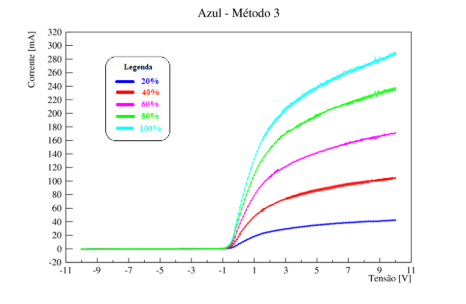
\includegraphics[scale=0.75]{figurateste.png} 
\caption{Legenda de la figura.} 
\label{fig:1} 
\end{figure}

\section{Análisis de Resultados}
Otro ejemplo es la figura \ref{fig:2}


\begin{table*}[ht]
\centering
\caption{Legenda de la tabla }
\label{tabladeseables}
\begin{tabular}{lcccccc}   \hline
Controlador  & $Re(\lambda)_{max}$  & $u_{max}$ & $t_{est}^{max}$ & $noise_{max}$ & $u_{nom}$ & $t_{est}^{nom}$  \\ \hline
PPGA23 & \textbf{AD} & \textbf{AD}& \textbf{AD}&\textbf{AD} &\textbf{AD} & \textbf{AD}\\
 \hline
 W34 & AD & AD & D & T & AD & IND \\
 \textbf{PPGA34} & \textbf{AD} & \textbf{AD} & \textbf{AD} & \textbf{AD} & \textbf{AD} & \textbf{AD} \\
  \hline
J45 & AD & IND & AD & IND & AD & AD \\
\textbf{PPGA23}**& \textbf{D} & \textbf{AD} & \textbf{D} & \textbf{T} & \textbf{AD} & \textbf{D} \\
 \hline
\end{tabular}
\end{table*}




% La extensión de la imagen debe ser png
\begin{figure}[H] 
\centering
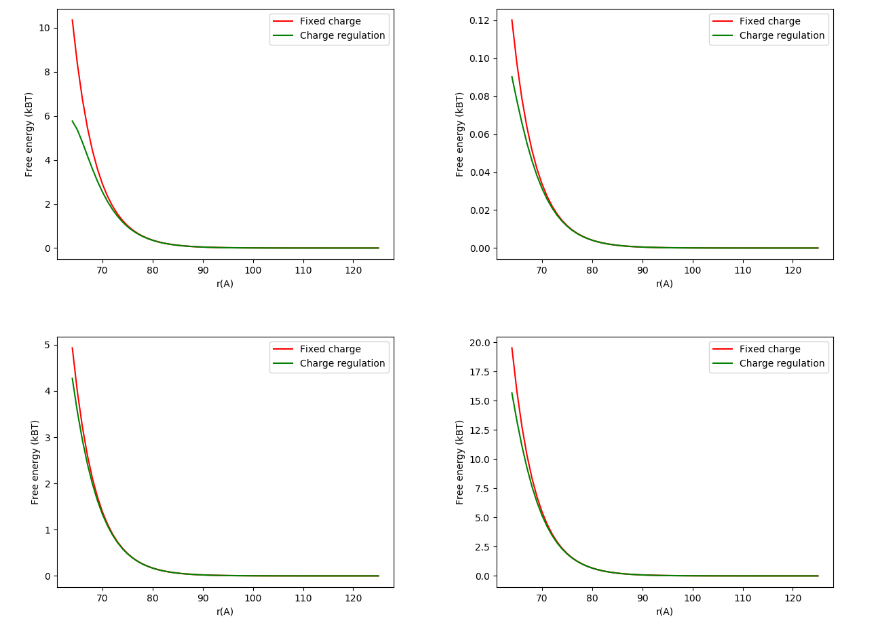
\includegraphics[scale=0.4]{figurateste2.png} 
\caption{Legenda de la figura.} 
\label{fig:2} 
\end{figure}


\section{Conclusiones}

Se resume lo que se obtuvo, si se llegó a lo deseado o no y las razones de ello.

\begin{thebibliography}{99}

\bibitem[1]{ref1} T. Dubos ,\textit{	Covariant Structure of Models of Geophysical Fluid Motion},
Phys. Rev. Lett. {\bf 120}, p. 2018 (2018).
\bibitem[2]{ref2} D. Coumou, G. Di Capua, S. Vavrus, L. Wang and S. Wang,\textit{The influence of Artic amplification on mid-latitude summer circulation},
Nature Communications  {\bf 9}, 2959 (2018).
\bibitem[3]{ref3} J. Francis and N. Skific,\textit{	Evidence linking rapid Arctic warming to mid-latitude weather patterns},
Philosophical Transactions of the Royal Society A: Mathematical, Physycal and Engineering Sciences  {\bf 373}, (2015).
 
\end{thebibliography}

\end{multicols}
\end{document}